\documentclass{article}
\usepackage{graphicx}

\setlength{\parindent}{0pt}
\setlength{\parskip}{5pt}

\begin{document}

\title{UADE 2.xx design specification}
\author{Heikki Orsila $<$heikki.orsila@iki.fi$>$}
\date{}
\maketitle

\section{Introduction}

\subsection{History}

UADE 1.xx was written to be a stand-alone program that had separate code
for each possible \emph{frontend} (\emph{user interface}), but there was
no internal structure to implement different frontends easily. By much
hacking some kind of pseudo-interface was created to facilitate following
frontends:
\begin{itemize}
  \item Beep Media Player
  \item MorphOS shell without interaction
  \item Unix shell without interaction
  \item Unix shell with small interaction
  \item XMMS plugin
\end{itemize}

It was a clear design problem that needed to be fixed. To force the separation
of frontend and \emph{uadecore} (emulator), UADE 2.xx removed all user
interface issues from the uadecore.

\subsection{Message-passing protocol}
In UADE 2.xx the emulator (uadecore) became an independent process without
any user interfaces. Any frontend, or client, that wants to use its services
must communicate with the uadecore by using a token-passing based messaging
protocol. The protocol is of course implemented by interprocess communication
(IPC).

The basic idea of the protocol is that the frontend is the client
who issues commands for the server (uadecore). Uadecore may not send any
commands at all. Uadecore only sends replies to commands issued by the
client. Also, the client never replies anything back to the
uadecore.

The communication protocol is based on the concept of
\emph{tokens}. Only the party that has a token (there is only one) may
send messages. Messages are either commands or replies. Client sends
messages and uadecore sends replies. Both of them have to send the token back
sometimes. The party that doesn't have the token must reply to all commands
sent by the other party.

The messaging protocol has following commands:

\begin{description}
\item [Config] command is used to pass a file name of the emulation
configuration file for the uadecore. The file is named \emph{uaerc}.

\item [Score] command is used to pass file name of a binary run-time in M68k
machine language for the uadecore. The binary run-time is called
\emph{score} or \emph{sound core}. The sound core contains implementations of
\emph{Eagleplayer} and \emph{AmigaOS} APIs.

\item [Player] command is used to pass a file name of a binary player plugin
in M68k machine language for the uadecore. This is also called an
\emph{Eagleplayer plugin}.

\item [Module] command is used to pass a file name of a song to be played
for the uadecore.

\item [Read] command is used to request more sound data from the uadecore.

\item [Reboot] command is used to halt playback synthesis of uadecore.

\item [Set subsong] command is used to set the initial subsong for playback.

\item [Ignore check] command is not necessary (will be documented later,
if ever).
\item [Song end not possible] command is not necessary.
\item [Set ntsc] command is not necessary.
\item [Filter] command is not necessary.
\item [Set interpolation mode] command is not necessary.
\item [Speed hack] command is not necessary.
\item [Change subsong] command is not necessary.
\item [Activate debugger] command is not necessary.

\item [Token] command is used to pass back the token for the other party.

\end{description}
Messages are answered by following replies:
\begin{description}
\item [MSG]
\item [Can't play]
\item [Can play]
\item [Song end]
\item [Subsong info]
\item [Player name]
\item [Module name]
\item [Format name]
\item [Data]
\end{description}.

\begin{figure}
\centering
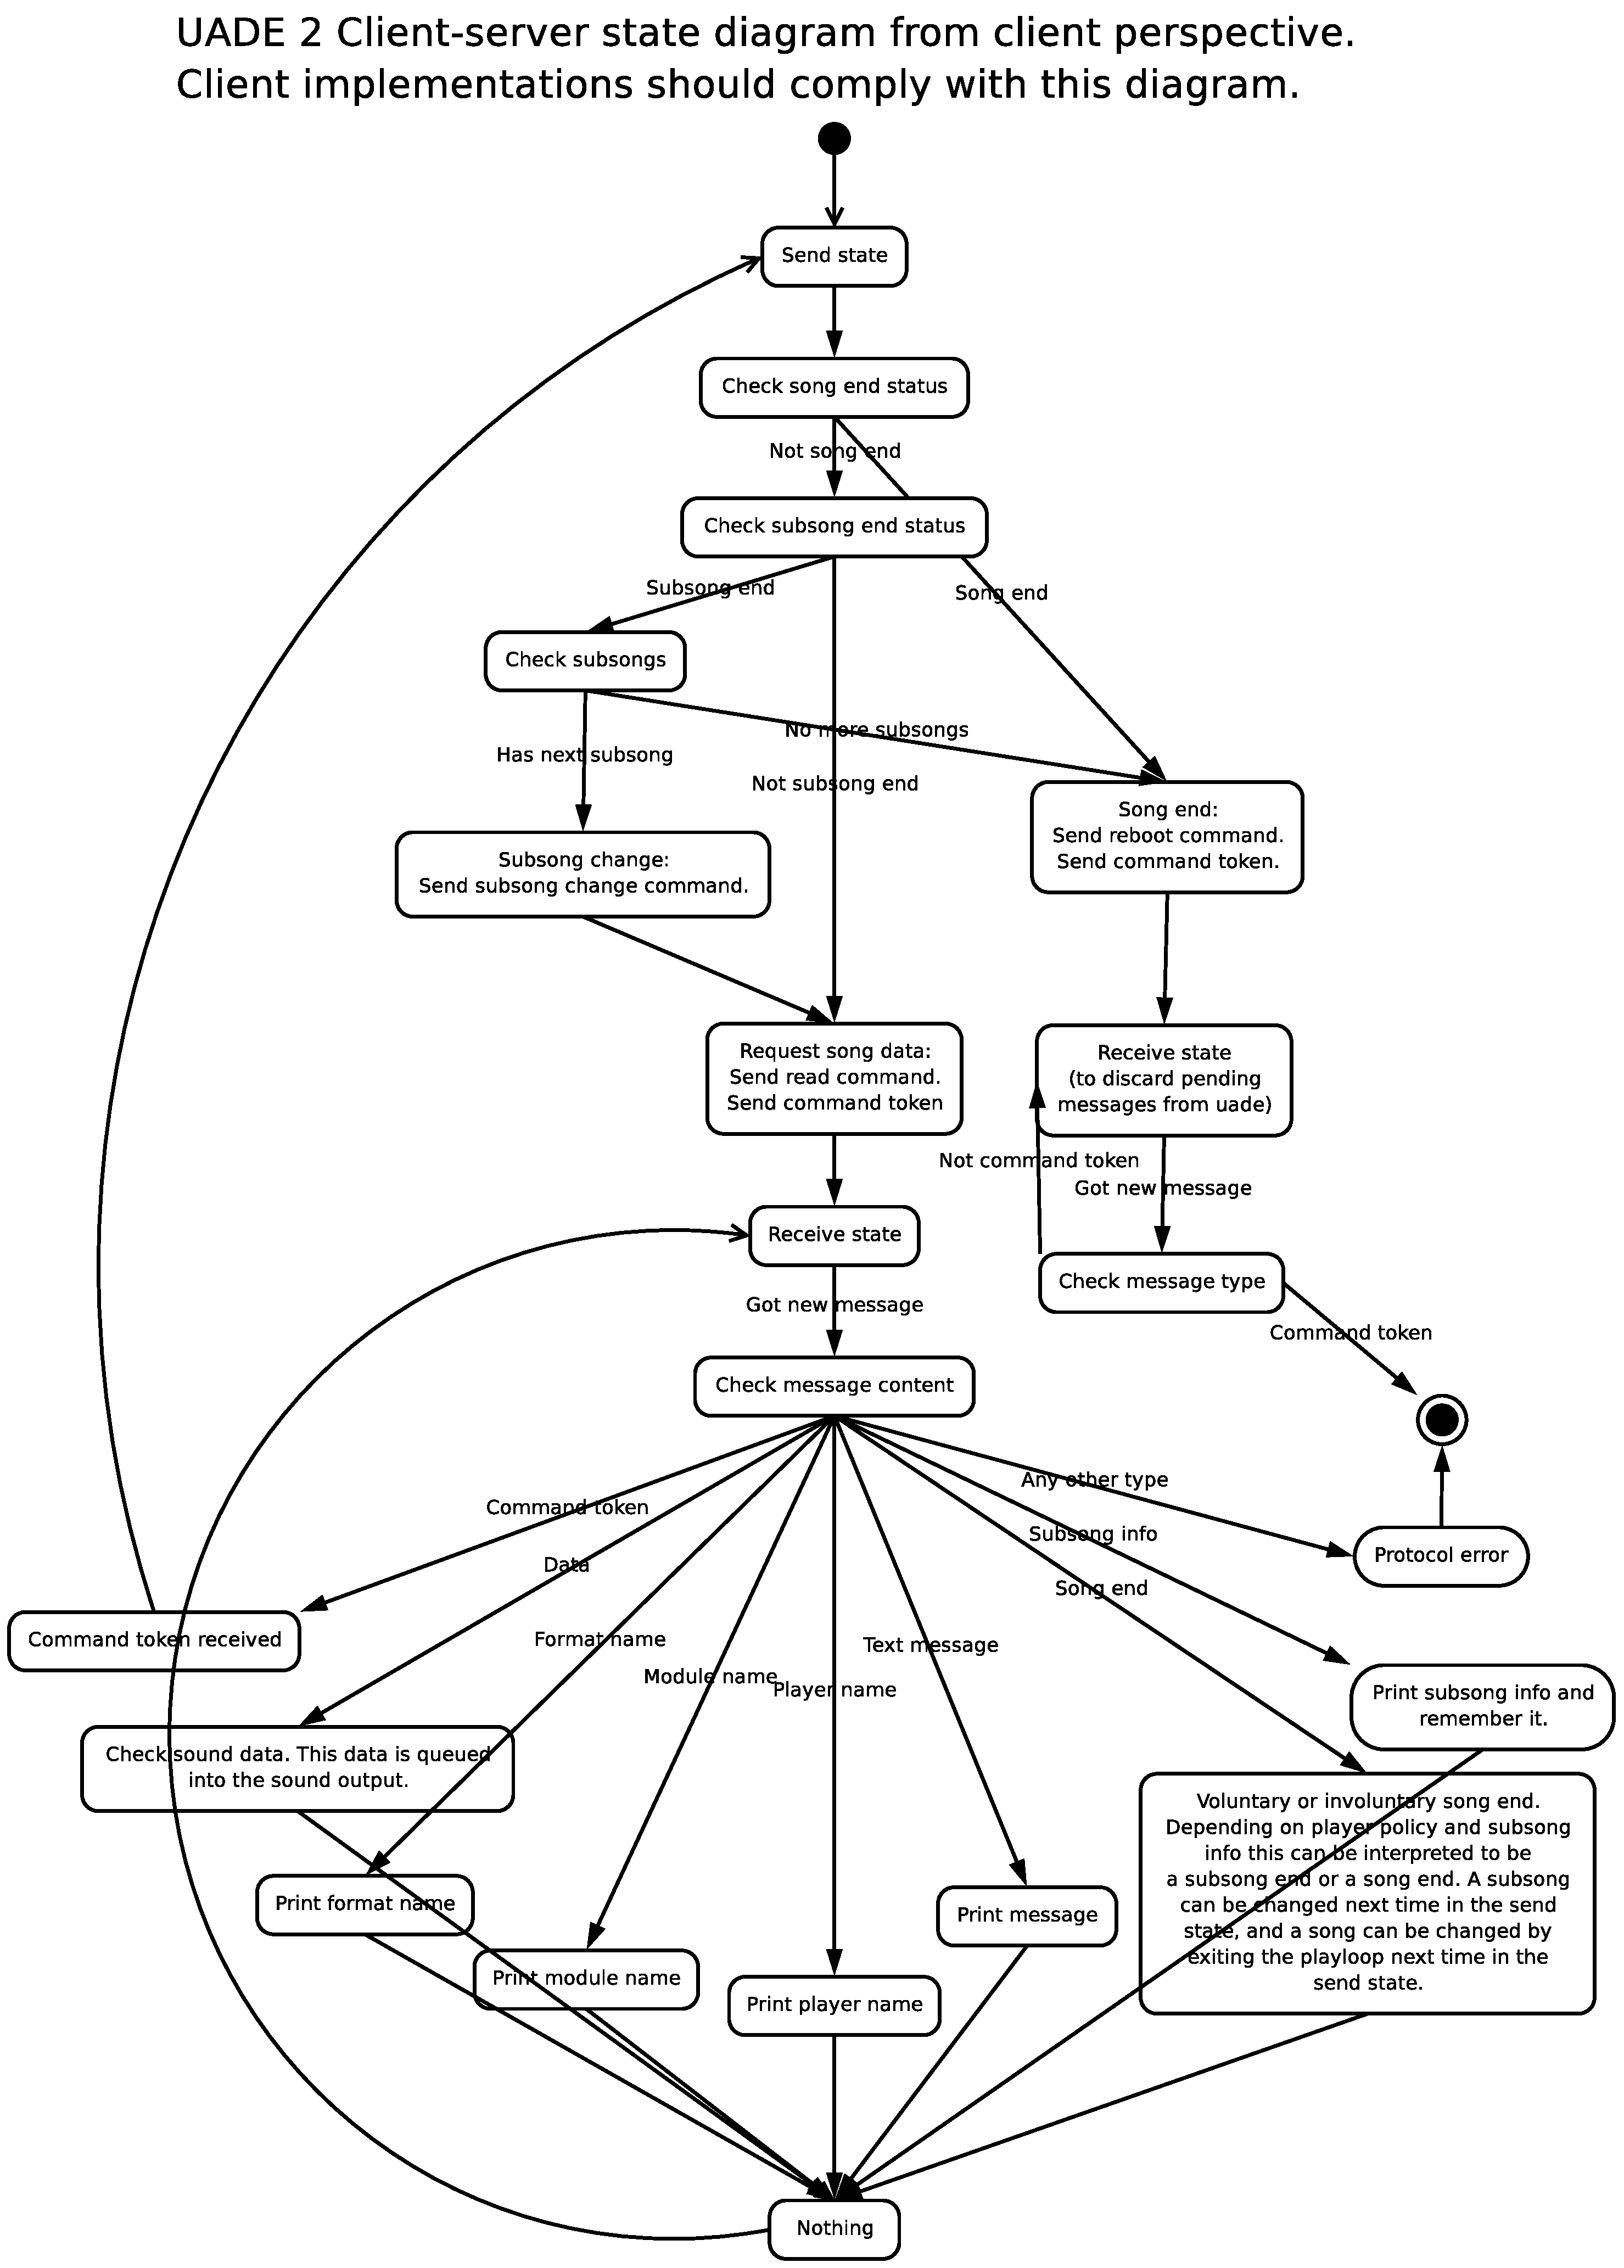
\includegraphics[scale=0.25]{play_loop_state_diagram.eps}
\caption{Play loop interaction from client (frontend) perspective}
\label{fig:playloop}
\end{figure}

\end{document}
